% This LaTeX document needs to be compiled with XeLaTeX.
\documentclass[
  10
]{article}
\usepackage[margin=2cm,includehead=true,includefoot=true,centering,]{geometry}
\usepackage{xcolor}
\usepackage{ucharclasses}
\usepackage{hyperref}
\usepackage{amsmath,amssymb}
\usepackage{amsfonts}
\usepackage[version=4]{mhchem}
\usepackage{stmaryrd}
\usepackage{bbold}
\usepackage{polyglossia}
\usepackage{fontspec}
\usepackage{ctex}
\usepackage[export]{adjustbox}
\usepackage{tabularx}
\usepackage{booktabs}

\usepackage{setspace}
\setstretch{1.2}

\makeatletter
\@ifundefined{KOMAClassName}{% if non-KOMA class
  \IfFileExists{parskip.sty}{%
    \usepackage{parskip}
  }{% else
    \setlength{\parindent}{0pt}
    \setlength{\parskip}{6pt plus 2pt minus 1pt}}
}{% if KOMA class
  \KOMAoptions{parskip=half}}
\makeatother
\usepackage{longtable,booktabs,array}
\newcounter{none} % for unnumbered tables
\usepackage{calc} % for calculating minipage widths
% Correct order of tables after \paragraph or \subparagraph
\usepackage{etoolbox}
\makeatletter
\patchcmd\longtable{\par}{\if@noskipsec\mbox{}\fi\par}{}{}
\makeatother
% Allow footnotes in longtable head/foot
\IfFileExists{footnotehyper.sty}{\usepackage{footnotehyper}}{\usepackage{footnote}}
\makesavenoteenv{longtable}
\usepackage{graphicx}
\makeatletter
\newsavebox\pandoc@box
\newcommand*\pandocbounded[1]{% scales image to fit in text height/width
  \sbox\pandoc@box{#1}%
  \Gscale@div\@tempa{\textheight}{\dimexpr\ht\pandoc@box+\dp\pandoc@box\relax}%
  \Gscale@div\@tempb{\linewidth}{\wd\pandoc@box}%
  \ifdim\@tempb\p@<\@tempa\p@\let\@tempa\@tempb\fi% select the smaller of both
  \ifdim\@tempa\p@<\p@\scalebox{\@tempa}{\usebox\pandoc@box}%
  \else\usebox{\pandoc@box}%
  \fi%
}
% Set default figure placement to htbp
\def\fps@figure{htbp}
\makeatother
\setlength{\emergencystretch}{3em} % prevent overfull lines
\providecommand{\tightlist}{%
  \setlength{\itemsep}{0pt}\setlength{\parskip}{0pt}}


\hypersetup{colorlinks=true, linkcolor=blue, filecolor=magenta, urlcolor=cyan,}
\urlstyle{same}

\usepackage{colortbl}
\definecolor{table-row-color}{HTML}{999999}
\definecolor{table-rule-color}{HTML}{999999}
%\arrayrulecolor{black!40}
\arrayrulecolor{table-rule-color}     % color of \toprule, \midrule, \bottomrule
\setlength{\aboverulesep}{0pt}
\setlength{\belowrulesep}{0pt}


\setotherlanguages{english}
\IfFontExistsTF{Source Han Serif CN}
{\newfontfamily\chinesefont{Source Han Serif CN}}
{\IfFontExistsTF{Noto Serif CJK SC}
  {\newfontfamily\chinesefont{Noto Serif CJK SC}}
  {\IfFontExistsTF{SimSun}
    {\newfontfamily\chinesefont{SimSun}}
    {\IfFontExistsTF{FangSong}
      {\newfontfamily\chinesefont{FangSong}}
      {\newfontfamily\chinesefont{Arial Unicode MS}}
}}}
\IfFontExistsTF{Times New Roman}
{\newfontfamily\englishfont{Times New Roman}}
{\IfFontExistsTF{Liberation Serif}
  {\newfontfamily\englishfont{Liberation Serif}}
  {\IfFontExistsTF{DejaVu Serif}
    {\newfontfamily\englishfont{DejaVu Serif}}
    {\newfontfamily\englishfont{Arial}}
}}


\author{}
\date{}

\begin{document}


\section{2025年金华婺城、金东小学六年级教育质量综合测评卷}\label{ux5e74ux91d1ux534eux5a7aux57ceux91d1ux4e1cux5c0fux5b66ux516dux5e74ux7ea7ux6559ux80b2ux8d28ux91cfux7efcux5408ux6d4bux8bc4ux5377}

(考试时间:90 分钟 满分:100 分) 2025 年 6 月考

班级：\_\_\_\_ 姓名：\_\_\_\_ 学号：\_\_\_\_

\subsection{一、填空题（第2题4分，其余每题2分，共26分）}\label{ux4e00ux586bux7a7aux9898ux7b2c2ux98984ux5206ux5176ux4f59ux6bcfux98982ux5206ux517126ux5206}

\begin{enumerate}
\def\labelenumi{\arabic{enumi}.}
\item
  太平洋是世界上最大的洋,
  它的面积约是一亿八千一百三十四万四千平方千米。横线上的数写作( ),
  四舍五入到亿位约是( )亿。
\item
  右图中涂色部分与整个图形的面积关系可以用下面的式子表示：
\end{enumerate}

( ) : \(8=\frac{(\quad)}{16}=12\div(\quad)=(\quad)\%\)

\pandocbounded{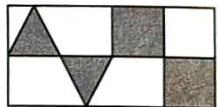
\includegraphics[keepaspectratio]{images/3bc4455833a7bb2be201888a245c4789fb76f8bd946b647e11e679f4c56188d2.jpg}}

3.用 36 个棱长为 \(1 \mathrm{~cm}\) 的小正方体搭成一个大长方体,
已知大长方体的底面是一个边长为 \(2 \mathrm{~cm}\) 的正方形,
则这个大长方体的高为 ( ) cm。

4.下面是2024全国游泳锦标赛女子50米蝶泳决赛成绩表,其中部分数字被遮挡。已知这三位运动员的比赛成绩非常接近,王一淳的成绩是(
)秒,张雨霏比王一淳快( )秒。

{\def\LTcaptype{none} % do not increment counter
\begin{longtable}[]{@{}|l|l|l|l|@{}}
\toprule\noalign{}
\endhead
\bottomrule\noalign{}
\endlastfoot
\hline
运动员 & 张雨霏 & 王一淳 & 余依婷 \\
\hline
成绩/秒 & ★5.16 & 2★.41 & 25.46 \\
\hline
奖牌 & 金牌 & 银牌 & 铜牌 \\
\hline
\end{longtable}
}

5.《水浒传》是我国四大古典名著之一,作者成功塑造了``水泊梁山108位好汉''的形象。108的因数有(
)个,从这个数的因数中选出4个数组成一个比例:( )。

\begin{enumerate}
\def\labelenumi{\arabic{enumi}.}
\setcounter{enumi}{5}
\tightlist
\item
  小红本次体育抽测的成绩是 91 分, 王老师将它记作 +3 分;
  小明的成绩单不小心被墨水弄脏了, 小明的体育抽测成绩可能 ( ) 分, 也可能
  ( ) 分。
\end{enumerate}

{\def\LTcaptype{none} % do not increment counter
\begin{longtable}[]{@{}|l|l|l|@{}}
\toprule\noalign{}
\endhead
\bottomrule\noalign{}
\endlastfoot
\hline
姓名 & 成绩 & 记作 \\
\hline
小红 & 91分 & +3分 \\
\hline
小明 & & 5分 \\
\hline
\end{longtable}
}

7.一幅地图的比例尺是0 40 80 120 km,把它改写成数值比例尺是(
);已知A、B两地在这幅地图上的距离是4.5 cm,A、B两地的实际距离是( )km。

\begin{enumerate}
\def\labelenumi{\arabic{enumi}.}
\setcounter{enumi}{7}
\tightlist
\item
  古希腊的毕达哥拉斯喜欢用石子摆数, 他发现当小石子的数量是
  \(1,3,6,10 \cdots\) 时, 都能摆成等边三角形。这样的数称为``三角形数'',
  如下图:
\end{enumerate}

\pandocbounded{
\includegraphics[keepaspectratio]{images/62006f0fb07b41752e321cd90d5492b9492ae4d0d5680388e86251585f1b53a3.jpg}}

natural\_image

Abstract pattern of black dots arranged in triangular clusters on white
background (no text or symbols)

(1)第6个三角形数是( )。

(2)观察图与数的关系,第( )个三角形数是36。

9.商家要给右面的箱子打包(单位:cm),其打包方式如图所示,则打包带的长度至少要(
)cm。(打结处忽略不计)

\pandocbounded{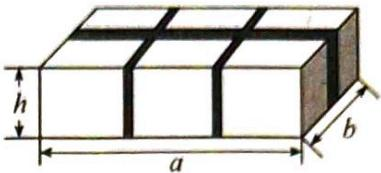
\includegraphics[keepaspectratio]{images/0484193d656bccda03512690ff1deec606cd9baf69c6248b3fe98c4fa4aa2776.jpg}}

text\_image

h a b

10.仔细观察下图中的3道计算题,整数、小数、分数加减法计算方法的相同点是(
)。

\begin{enumerate}
\def\labelenumi{(\arabic{enumi})}
\item
  \(\frac{+165}{199}\) 个位对齐(2)
  \(\frac{-2}{1}\cdot\frac{1}{5}\cdot\frac{2}{8}\) 小数点对齐
\item
  \(\frac{1}{2}+\frac{3}{8}=\boxed{\frac{4}{8}+\frac{3}{8}}=\frac{7}{8}\)
  通分
\end{enumerate}

\begin{enumerate}
\def\labelenumi{\arabic{enumi}.}
\setcounter{enumi}{10}
\item
  学校组织看了神舟十九号载人飞船发射后, 淘气打算用一块棱长为
  \(6 \mathrm{~cm}\)
  的正方体橡皮泥做一个由等底等高的圆柱和圆锥组合而成的最大``火箭''模型,
  其中圆锥的体积是 \((\quad)\mathrm{cm}^{3}\) , 圆柱的体积是
  \((\quad)\mathrm{cm}^{3}\) 。
\item
  李老师正在上传一份大小为 860 MB 的文件。页面显示已经上传了 40\%, 用时
  1 分 26 秒。这份文件已经上传了( )MB。照这样的速度, 上传完整份文件,
  一共需要( )秒。
\end{enumerate}

\pandocbounded{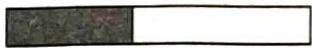
\includegraphics[keepaspectratio]{images/96073a85a1c334c54cd833b55a16c258fbca79ffe3a4d4eb4e5293cc1ca83a59.jpg}}

状态：正在上传中\ldots\ldots{} 已上传：40\%

\subsection{二、选择题(每题1分,共10分)}\label{ux4e8cux9009ux62e9ux9898ux6bcfux98981ux5206ux517110ux5206}

\begin{enumerate}
\def\labelenumi{\arabic{enumi}.}
\tightlist
\item
  下列百分率中, 可能超过 \(100\%\) 的是( )。
\end{enumerate}

A. 种子的成活率

B. 一次测试的及格率

C. 销售量的增长率

D. 大豆的出油率

2.世界上最大的立体造型温度计是我国新疆吐鲁番火焰山的``金箍棒''。程程去旅游时为了知道``金箍棒''的高度,测量了同一时刻他自己和``金箍棒''的影长,程程的影长是34厘米,``金箍棒''的影长是240厘米。已知程程的身高为1.7米,则``金箍棒''高(
)米。

A. 1.2

B. 12

C. 4.8

D. 48

3.如图,图②是将图①中半圆 BMO 以点 O 为中心旋转得到的。若 AO=10
cm,则图①中涂色部分的周长是( )cm。

\pandocbounded{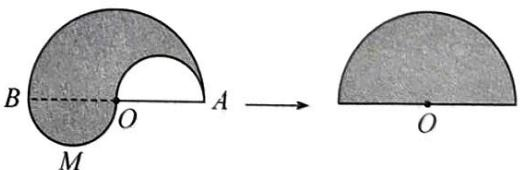
\includegraphics[keepaspectratio]{images/bf8f48e9b6fa1d4c331ad97c20703d0ee8840ba58cfd33fe0580090422343383.jpg}}

text\_image

B O A M → O

B. 31.4

图①

图②

A. 62.8

C. 51.4

D. 41.4

4.前两天,王叔叔网购了一件商品,今天收到快递。快递包装箱的尺寸是
\(7 \mathrm{dm} \times 6 \mathrm{dm} \times 15 \mathrm{dm}\) 。它可能是(
)。

A. 手机

B. 笔记本电脑

C. 鞋子

D. 冰箱

5.用四根木条制作一个长方形框架,将它的两个对角慢慢向两边拉动,每次拉动形成的平行四边形的面积和高()。

\pandocbounded{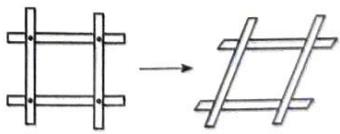
\includegraphics[keepaspectratio]{images/08ca1005d8757a4dda549cb29e48c15bd32f96c031d90a972e9f77c2b7eb28ca.jpg}}

natural\_image

Diagram showing two structural frame arrangements, one with vertical
supports and one with horizontal beams, both without any text or
symbols.

A. 成正比例

B. 成反比例

C.不成比例

D. 可能成正比例也可能成反比例

6.冬至是一年中黑夜最长、白昼最短的一天。2024年冬至是12月21日，某市日出时间是7:33，日落时间是16:53。下面表述错误的是（
）。

A. 冬至这天该市黑夜时间与白昼时间的比是 11:7

B. 冬至这天该市黑夜时间比白昼时间多 \(\frac{4}{11}\)

C. 冬至这天该市白昼时间占全天时间的 \(\frac{7}{18}\)

D. 冬至这天该市黑夜时间约占全天时间的 \(61\%\)

7.下面的图和算式,其中画方框部分表示0.6的是()。

\pandocbounded{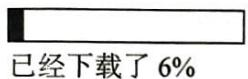
\includegraphics[keepaspectratio]{images/67d37fac85333406bc5ae104c8f157bdce9d375a855b7ffa10067f9cae01bb54.jpg}}\\
A.

\pandocbounded{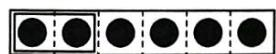
\includegraphics[keepaspectratio]{images/c9589e7f11691f9b7273eb3ed70ce7073fc373adc0a7720c7c46f1b2ab8f3e9c.jpg}}\\
B.

\pandocbounded{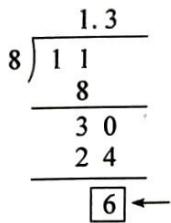
\includegraphics[keepaspectratio]{images/bc2b664c1474b5b025f9c48ad3a705c33543e483bf22ed68564b178feb26c97c.jpg}}\\
C.

\pandocbounded{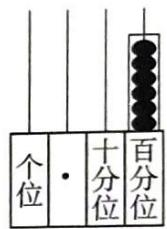
\includegraphics[keepaspectratio]{images/c186230c59f1bbbbbc5a5e35dc613ac0299d44b6cc9f6aac86a3814a4d8f7b6e.jpg}}\\
D.

8.如图,用 8
个完全相同的小长方形可以拼成一个大长方形,每个小长方形的面积是( )cm²。

\pandocbounded{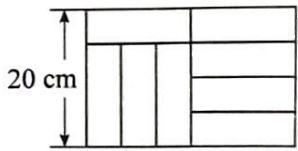
\includegraphics[keepaspectratio]{images/cc9f183e776af6cb931652416d1017a567a62ecc3e7460f4d820564eb8cf490c.jpg}}

text\_image

20 cm

A. 96

B. 75

C. 50

D. 64

\begin{enumerate}
\def\labelenumi{\arabic{enumi}.}
\setcounter{enumi}{8}
\tightlist
\item
  黑色袋子里有红、黄两种颜色的球各 3 个(除颜色外完全相同),
  要想保证摸出的球中一定有两个是同色的, 则摸出球的个数至少有( )个。
\end{enumerate}

A. 2

B. 3

C. 4

D. 5

10.下面说法错误的有( )个。

①在折线统计图中,折线越缓,说明数据的变化越大;折线越陡,说明数据的变化越小。

②3:4 的前项加上 9, 要使比值不变, 后项应该加上 12。

③连续的两个月最多有62天,最少有58天。

④一种体育彩票的中奖率是1\%，小李买了100张彩票，一定会有1张中奖。

A. 1

B. 2

C. 3

D. 4

\subsection{三、计算题(26 分)}\label{ux4e09ux8ba1ux7b97ux989826-ux5206}

\begin{enumerate}
\def\labelenumi{\arabic{enumi}.}
\tightlist
\item
  直接写出得数。(每题 1 分, 共 8 分)
\end{enumerate}

\[
1. 2 \times 0. 6 =
\]

\[
0. 5 ^ {2} - 0. 3 ^ {2} =
\]

\[
\frac {2}{8} + \frac {5}{8} \times 0 =
\]

\[
2. 5 \times 0. 4 \div 2. 5 =
\]

\[
2 3. 9 \div 8. 1 \approx
\]

\[
3 5 \pi \div 5 \pi =
\]

\[
4 2 \div 0. 3 =
\]

\[
1 + 20 \% - 30 \% =
\]

2.用递等式计算。(每题3分,共12分)

\[
\frac {8}{9} \times \frac {2}{5} \div \frac {8}{1 5}
\]

\[
\frac {3}{5} \times 2 4 + 7 \times 0. 6 - \frac {3}{5}
\]

\[
9. 8 3 - (4. 9 3 + 2 \frac {1}{4})
\]

\[
2 4 \div (\frac {5}{1 2} - \frac {3}{8}) \times \frac {1}{4 8}
\]

\begin{enumerate}
\def\labelenumi{\arabic{enumi}.}
\setcounter{enumi}{2}
\tightlist
\item
  解方程或比例。(每题 2 分, 共 6 分)
\end{enumerate}

\[
\frac {2}{3} x - 1 4 = 4
\]

\[
\frac {1}{2}: \frac {1}{6} = x: 1. 2
\]

\[
6 0 + 5 x = 9 0
\]

\subsection{四、操作与分析(11
分)}\label{ux56dbux64cdux4f5cux4e0eux5206ux679011-ux5206}

\begin{enumerate}
\def\labelenumi{\arabic{enumi}.}
\tightlist
\item
  按要求画图。(4 分)
\end{enumerate}

(1)把图中的长方形绕点 A 逆时针旋转 \(90^{\circ}\)
，画出旋转后的图形。旋转后点 B 的位置用数对表示是（，）。

(2)画出一个与长方形面积相等的三角形。如果按 2:1 的比将三角形放大,
放大后的三角形与原来三角形的面积比是( )。

2.根据要求,画出到点 A 的距离等于 3 厘米的所有的点。(2 分)

\pandocbounded{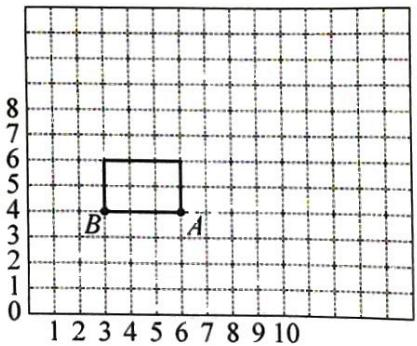
\includegraphics[keepaspectratio]{images/fde433812efadcc9460f1951b4f08356bc88b07c52bc45d860fe00a72b4e6c38.jpg}}

text\_image

B A

\pandocbounded{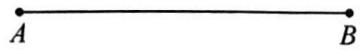
\includegraphics[keepaspectratio]{images/dacea564e21f54227d48ac745f5022374342ae8709c559e90e8fd4c6f4140a33.jpg}}

\begin{enumerate}
\def\labelenumi{\arabic{enumi}.}
\setcounter{enumi}{2}
\tightlist
\item
  求出右面图形的体积。(单位: cm)(3 分)
\end{enumerate}

\pandocbounded{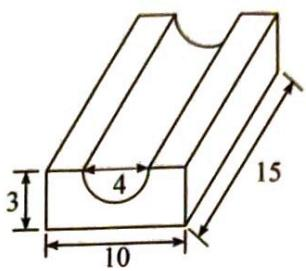
\includegraphics[keepaspectratio]{images/c34b40af885bc916ccb31a4264140eb7dc1c4f7ed1a14dd5cb99f66198d1d132.jpg}}

text\_image

3 4 10 15

\begin{enumerate}
\def\labelenumi{\arabic{enumi}.}
\setcounter{enumi}{3}
\tightlist
\item
  小探究: 你能比较 \(16 \times 28\) 和 \(18 \times 26\)
  的乘积谁大谁小吗? 笑笑这样想:
\end{enumerate}

\[
\boxed {\begin{array}{l}1 6 \times 2 8 = 1 6 \times (2 6 + 2) = 1 6 \times 2 6 + 1 6 \times 2 \text {小}\\1 8 \times 2 6 = (1 6 + 2) \times 2 6 = 1 6 \times 2 6 + 2 \times 2 6 \text {大}\end{array}} \rightarrow \boxed {1 6 \times 2 8 <   1 8 \times 2 6}
\]

请你也像笑笑那样,分析 \(71 \times 34\) 和 \(69 \times 36\)
的乘积谁大谁小。(2 分)

\subsection{五、解决问题(27分)}\label{ux4e94ux89e3ux51b3ux95eeux989827ux5206}

1.为了预防感冒,某学校六(1)班老师用13升姜汁加水调制了55升姜汤。校医说:``当姜汁和水的比是3:7时,效果最佳。''为了使调制的姜汤效果最佳,应该再往调制的姜汤中加多少升姜汁?(4分)

2.六一儿童节,爸爸送给张伟一个圆锥形的玩具(如右图),如果要用一个长方体的盒子包装它,这个盒子的表面积至少是多少平方厘米?(4分)

\pandocbounded{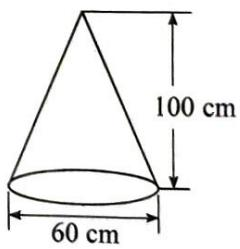
\includegraphics[keepaspectratio]{images/40ee3a26029da96800ac79eae99a5562d08041c91c4d2e16e988a65d681abd88.jpg}}

text\_image

100 cm 60 cm

\begin{enumerate}
\def\labelenumi{\arabic{enumi}.}
\setcounter{enumi}{2}
\tightlist
\item
  萍萍和爸爸、妈妈一起去看电影, 电影票原价 45 元/张
  (成人和儿童的票价相同), 经比较以后, 他们选择了有优惠的场次,
  三张票共节省了 27 元。他们看的是哪一场? (4 分)
\end{enumerate}

{\def\LTcaptype{none} % do not increment counter
\begin{longtable}[]{@{}|l|l|@{}}
\toprule\noalign{}
\endhead
\bottomrule\noalign{}
\endlastfoot
\hline
\multicolumn{2}{@{}l@{}}{%
优惠方式} \\
\hline
上午场(9:00---11:00) & 六折 \\
\hline
下午场(13:00---15:00) & 八折 \\
\hline
其他时段 & 原价 \\
\hline
\end{longtable}
}

4.金华市青少年乒乓球锦标赛使用36张球桌进行比赛,其中单打和双打同时进行,现场共有118名运动员参与比赛。请问:有几张桌是单打,几张桌是双打?(4分)

5.如图，张叔叔从A市途经B城匀速驾车到C市。

\pandocbounded{
\includegraphics[keepaspectratio]{images/ba50d98043f6d08d36146dc6419edfc720e4cc2afced600e75edc5bc78bf329c.jpg}}

信息 1: A、B 两地与 B、C 两地的路程比是 4:3;

信息 2: 张叔叔从 A 市出发, 以 80 km/h 的速度行驶了 2.5 小时到达 B 城。

信息 3: 当汽车行驶 20 km 时, 耗油量是 2.4 L。

信息 4: 张叔叔到达 B 城后, 休息 1.5 小时继续驾车向 C 市出发。

(1)A市到C市的路程是多少千米？(2分)

(2)假设每千米的耗油量不变,当耗油量达到30
L时,这辆汽车行驶了多少千米?(3分)

\begin{enumerate}
\def\labelenumi{\arabic{enumi}.}
\setcounter{enumi}{5}
\tightlist
\item
  下图是反映芳芳家平均每月家庭支出情况的不完整统计图。(6 分)
\end{enumerate}

芳芳家平均每月家庭支出情况扇形统计图

\pandocbounded{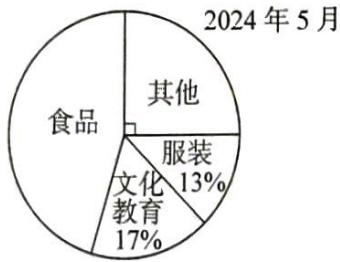
\includegraphics[keepaspectratio]{images/c0459cb5370b5901d8861df3e8e2ffb3ee36a9f0498d351793d9b171ea2ffed6.jpg}}

pie chart

2024年5月 \textbar{} Category \textbar{} Percentage (\%) \textbar{}
\textbar-\/-\/-\textbar-\/-\/-\textbar{} \textbar{} 食品 \textbar{} 17
\textbar{} \textbar{} 文化教育 \textbar{} 13 \textbar{} \textbar{} 服装
\textbar{} 13 \textbar{} \textbar{} 其他 \textbar{} 0 \textbar{}

芳芳家平均每月家庭支出情况条形统计图

\pandocbounded{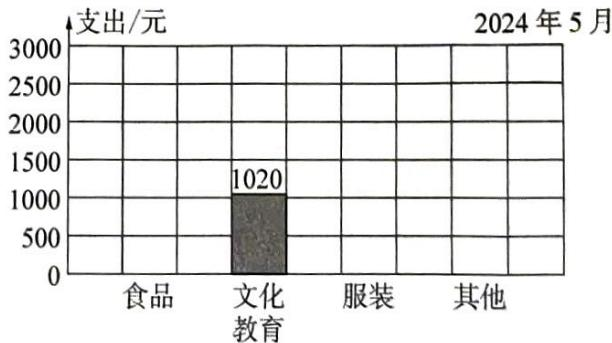
\includegraphics[keepaspectratio]{images/71a5326388becf338d4a585f3c5d479d4f93bb0297995891f610e5337f667b4f.jpg}}

bar chart

2024年5月 \textbar{} 类别 \textbar{} 支出/元 \textbar{}
\textbar-\/-\/-\textbar-\/-\/-\textbar{} \textbar{} 食品 \textbar{} 0
\textbar{} \textbar{} 文化教育 \textbar{} 1020 \textbar{} \textbar{}
服装 \textbar{} 0 \textbar{} \textbar{} 其他 \textbar{} 0 \textbar{}

(1)芳芳家平均每月家庭总支出是( )元。(1分)

(2)根据以上信息,将条形统计图补充完整。(3分)

(3)国际上通常用食品支出占家庭总支出的百分比(即恩格尔系数)来衡量一个地区的人民生活水平,如下表:

{\def\LTcaptype{none} % do not increment counter
\begin{longtable}[]{@{}|l|l|l|l|l|@{}}
\toprule\noalign{}
\endhead
\bottomrule\noalign{}
\endlastfoot
\hline
恩格尔系数 & 59\%以上 & 50\%\textasciitilde59\% &
40\%\textasciitilde50\% & 40\%以下 \\
\hline
生活水平 & 贫困 & 温饱 & 小康 & 富裕 \\
\hline
\end{longtable}
}

参照恩格尔系数,芳芳家处于什么生活水平?(在正确答案后面的□里画``√'')(2分)

贫困□ 温饱□ 小康□ 富裕□

\end{document}
